\section{Teoretická časť}

\subsection{Odporúčacie systémy}
 Vo všeobecnosti odporúčacie systémy sú algoritmy, ktorých hlavným cieľom, je odporučiť používateľovi jemu relevantné položky (filmy na pozretie, text na čítanie, produkty na kúpenie alebo čokoľvek iné v závislosti od odvetvia). Keď sa pozrieme na dôležitosť týchto systémov, v určitých odvetviach sú skutočne nevyhnutné, pretože môžu ,ak pracujú efektívne, pomáhať generovať firmám väčšie príjmy a navyše môžu predstavovať spôsob, ako vyniknúť oproti konkurencií a zlepšiť UX. Pri odporúčacích systémoch existujú dve hlavné techniky návrhu algoritmu a to tzv. collaborative filtering a content based filtering. Poďme sa teda pozrieť na rôzne koncepty týchto dvoch techník. \\

\subsubsection{Collaborative filtering}
Collaborative filtering je metóda vytvárania automatických predpovedí o záujmoch používateľa zbieraním preferencií od väčšieho počtu použivateľov. Základným predpokladom tejto metódy je, že ak používateľ A má rovnaký názor na produkt ako používateľ B, je vysoko pravdepodobné, že použivateľ A bude mať na iný produkt ten istý názor ako použivateľ B. Týmto postupom by systém vedel napríklad predpovedať, ktoré televízne šou ma daný používateľ rád, na základe jeho doterajších názorov (napr. vo forme likes/dislikes). Treba poznamenať, že tieto predpovede sú špecifické pre daného používateľa, ale vytvárajú sa na základe informácií zhromaždených od veľkého počtu iných používateľov. 

Hlavnou výhodou tejto metódy je, že sa časom s pribudajúcim počtom interakcií zlepšuje a stáva sa efektívnejšou. Avšak, vzhľadom nato, že berie do úvahy iba interakcie z minulosti, jej hlavným problémom je tzv. "cold start problem": znamená, že je takmer nemožné niečo odporučiť novému používateľovi, alebo odporúčať nový produkt používateľom, pokiaľ či už používateľ alebo produkt nemájú žiadne interakcie. Navyše mnoho používateľov a produktov má príliš málo interakcií nato, aby algoritmus s nimi vedel na začiatku efektívne pracovať. Riešenia tohto problému bývajú, že novým používateľom sa odporúčaju náhodné produkty a nové produkty sa odporúčajú náhodným používateľom (tzv. "random strategy"), odporúčanie populárnych produktov novým používateľom a odporúčanie nových produktov najviac aktivným používateľom (tzv. "maximum expectation strategy"). Tak isto sa často používa, že v skorej fáze "života" používateľa alebo produktu sa použije iná metóda ako collaborative filtering. \\\\

\begin{figure}[!htbp]
  \centering  
  \def\stackalignment{c}
	\stackunder{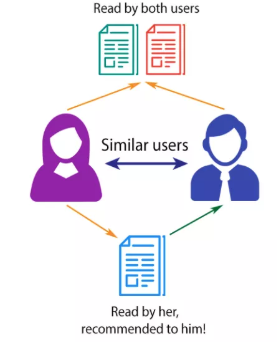
\includegraphics[width=7cm]{img/colaborative filtering.png}}%
           {\scriptsize%
            Zdroj: \url{https://towardsdatascience.com/the-remarkable-world-of-recommender-systems-bff4b9cbe6a7}}
  \caption{Collaborative filtering}
  
  \label{collaborativeFiltering}
\end{figure}

Existujú dva prístupy k tejto metóde.

\begin{enumerate}
	{\bf \item Memory-based methods} niekedy označované aj ako neighbourhood-based collaborative filtering algoritmy, v ktorých hodnotenia produktov používateľom sú predpovedané na základe jeho susedov. Týchto susedov môžeme ďalej definovať dvoma spôsobmi:
\begin{itemize}[leftmargin=*]
	{\bf \item User-based collaborative filtering:}\newline
Nájsť iných podobných používateľov a odporúčať produkty ktoré sa páčia im.
	{\bf \item Item-based collaborative filtering:}\newline
Odporúčať produkty ktoré používatelia označili, že sa im páčia, pričom niektoré iné produkty máte spoločne označené.
\end{itemize}
	{\bf \item Model-based methods} využívajú metódy strojového učenia na tvorbu predpovedí, pričom tento problém považujú ako normálny problém strojového učenia. Využívajú sa techniky ako PCA, SVD, faktorizácia matíc, clusterin či neurónové siete.
\end{enumerate}
 
\subsubsection{Content based filtering}
Táto metóda zahŕňa odporúčanie produktov na základe ich samotných vlastností. Odporúčania sú tu vytvárané na základe predchádzajúcich interakcií jednotlivého používateľa s produktami. Systém pracujúci touto metódou, sa snaží hladať podobnosti medzi produktami, s ktorými mal používateľ v minulosti pozitívnu interakciu (t.j. kúpil si daný produkt, ohodnotil kladne daný film, pridal skladbu do obľúbených atď.). Napríklad ak si používateľ v internetovom obchode s knihami kúpi knihu ktorá patrí do kategórie ‘literatúra’, je logické mu odporučiť knihy v tej istej alebo podobnej kategórii. Tak isto odporučiť mu knihy z toho istého roku vydania, alebo od toho istého autora. Výhodou content-based filteringu je, že nepotrebujeme veľa interakcií z minulosti nato, aby navrhoval relevantné produkty. Oproti tomu nevýhodou je, že sa systém časom neučí z interakcií a tým pádom sa ani časom nezlepšuje, keďže sa striktne drží informácií ktoré má o danom používateľovi. Ľudia sú však nepredvídateľní a ich vkus sa časom mení, preto v tomto ohľade má collaborative filtering navrch.
\begin{figure}[!htbp]
  \centering  
  \def\stackalignment{c}
	\stackunder{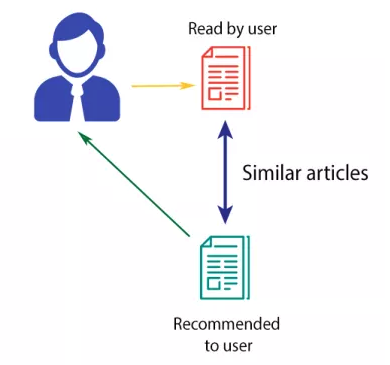
\includegraphics[width=7cm]{img/content-based-filtering.png}}%
           {\scriptsize%
            Zdroj: \url{https://towardsdatascience.com/the-remarkable-world-of-recommender-systems-bff4b9cbe6a7}}
  \caption{Content based filtering}
  
  \label{contentFiltering}
\end{figure}	

\subsection{Mobilné aplikácie}
Mobilná aplikácia je softvérová aplikácia vytvorená špecificky pre mobilné zariadenia ako napríklad smartfóny, tablety alebo inteligentné hodinky. Pôvodne boli aplikácie vytvárané výrobcami mobilných operačných systémov, ktorí potrebovali pre používateľov zjednodušiť používanie základných funkcií smartfónu, ako napríklad prezeranie emailov, správ o počasí, prácu s kalendárom, fotenie fotografií atď. Avšak, vďaka rýchlemu vývinu samotných smartfónov a ich operačných systémov, začal rásť dopyt aj po aplikáciách zameraných na iné oblasti. V dnešnej dobe sú najpopulárnejšie rôzne herné aplikácie, navigačné aplikácie, aplikácie na online komunikáciu, hudobné aplikácie a mnohé iné. V posledných rokoch si používanie smartfónu bez spomenutých aplikácií ani nevieme predstaviť a stali sa ich neoddeliteľnou súčasťou. Aplikácie sa väčšinou sťahujú z distribučných platforiem, ktoré sú prevádzkované vlastníkom daného operačného systému, na ktorý je aplikácia určená. Spomeniem dva najväčšie a to App Store patriaci pod operačný systém iOS a Google Play Store patriaci pod Android. Na oboch platformách vieme nájsť veľké množstvo aplikácií všemožného zamerania, pričom každým dňom pribúdajú ďalšie. Niektoré sú bezplatné, iné spoplatnené tvorcom, pričom zárobok z nej sa delí medzi tvorcu aplikácie a distribučnú platformu. 
\subsubsection{Typy mobilných aplikácií}
\begin{itemize}[leftmargin=*]
{\bf \item Natívne aplikácie} - sú vytvorené výlučne pre špecifický mobilný operačný systém tj. napríklad natívne Android aplikácie alebo natívne iOS aplikácie. Kvôli špecifickému zameraniu na jeden operačný systém nie je možné aplikácie kombinovať na rôznych platformách. Napríklad Blackberry aplikácia nie je spustiteľná na Androide, Windows Phone aplikáciu zase nespustíte na iOS. Teda všeobecne povedané, mobilnú aplikáciu nainštalujete a spustíte len na operačnom systéme, pre ktorý je vytvorená. Inštalujú sa priamo do mobilného zariadenia, potrebné dáta sú väčšinou uložené priamo v internom úložišku zariadenia. \\

{\bf Používané technológie:} Natívne aplikácie sú programované viacerými programovacími jazykmi. Medzi najpoužívanejšie patria Java, Kotlin, Python, Swift, Objective-C, C++ a React. \\

{\bf Výhody:} Vďaka tomu, že sú zamerané na jednu platformu, vedia byť z hľadiska výkonu rýchlejšie a stabilnejšie. Tiež majú vyššiu efektivitu pri využívaní samotného hardweru zariadenia. Sú prepojené priamo na hardware zariadení, čo im umožňuje mať možnosť využiť širokú ponuku funkcií, ktoré dané zariadenie ponúka ako napríklad fotoaparát, kontakty zariadenia, bluetooth, NFC či dokonca samotnú polohu zariadenia. Veľku obľubu im zabezpečuje aj to,  že využívajú natívny UI, čo prináša používateľom lepší UX. Niektoré nevyžadujú na funkčnosť internetové pripojenie. \\
 
{\bf Nevýhody:}  Primárnym problémom je duplicita pri vývoji aplikácie, keďže je potrebné aplikáciu naprogramovať pre viaceré mobilné operačné systémy, čo priamoúmerne zvyšuje cenu nehovoriac o náročnosti údržby a aktualizácie kódu pri každej novej verzii. Menší komfort spôsobuje aj fakt, že pri každej aktualizácií si používateľ musí aplikáciu preinštalovať resp. si nainštalovať tzv. update. \\

{\bf \item Webové aplikácie} - často sa správajú podobne ako natívne aplikácie, najpodstatnejší rozdiel je v tom, že sa k nim pristupuje pomocou webového prehliadača. Sú to v podstate responzívne webové stránky, ktoré sa prispôsobujú svojim vzhľadom zariadeniu na ktorom sú spustené. \\

{\bf Používané technológie:} Webové aplikácie sú vytvorené pomocou HTML (Hypertext Markup Language) ktorého vzhľad je naštýlovaný pomocou CSS (Cascading Style Sheet) a extra funkčnosť väčšinou zabezpečuje JavaScript. \\

{\bf Výhody:} Keďže na svoje fungovanie využívajú webový prehliadač, v tomto prípade zaniká problém duplicity pri programovaní aplikácie na viaceré operačné systémy. Toto znižuje náročnosť či už na vývoj, alebo cenu. Navyše odpadá potreba sťahovania, inštalácie a aktualizovania čo znamená, že aplikácia nezaberie žiadny priestor v úložisku zariadenia.  \\
 
{\bf Nevýhody:}  Hlavná nevýhoda pramení už z názvu - webové aplikácie, z čoho vyplýva, že sú závislé od internetového pripojenia. Webový prehliadač vie tiež zohrať veľkú rolu pri používaní týchto aplikácií. Kým v jednom môže byť k dispozicií plná funkcionalita, môže sa stať, že na druhom už len obmedzená čo môže znepríjemniť UX. Programátori sa tomu samozrejme snažia zabrániť a programovať aplikácie tak, aby boli plne funkčné na čo najväčšom množstve najviac používaných prehliadačov. \\
 
{\bf \item Hybridné aplikácie} - sú založené na pincípe miešania prvkov natívnych a webových aplikácií. Jadro aplikácie je napísane pomocou webových technológií (HTML, CSS, JavaScript), pričom je spúšťané z natívnej aplikácie a jej vlastného zabudovaného prehliadača, ktorý je ale pre používateľa neviditeľný. Napríklad aplikácia pre iOS by na zobrazenie používala WKWebView objekt, zatiaľ čo v Androide by na vykonávanie rovnakej funkcie používala WebView objekt. Kód samotný je potom vložený do kontajnera natívnej aplikácie s použitím frameworkov ako Apache Cordova (zámy aj ako PhoneGap), alebo Ionic. Tieto frameworky navyše majú aj systém pluginov, ktorý umožňuje ľahko prekonať obmedzenia webových aplikácií a rozšíriť funkcionalitu za rámec prehľadávača. Aplikácia tak môže získať plnú kontrolu nad funkciami mobilného zariadenia, čo umožňuje napríklad použiť TouchID pri iOS ako možnosť prihlásenia do aplikácie. Druhý možný spôsob fungovania aplikácie, ktorý je v posledných rokoch na vzostupe je, že aplikácie su kompilované do natívneho kódu. Využívajú ho frameworky ako React Native alebo NativeScript. Viac o React Native si povieme v ďalšej kapitole.\\


{\bf Používané technológie:} Hybridné aplikácie používajú kombináciu webových technológií a natívnych API. Sú vyvinuté pomocou technoĺogií ako Ionic, Apache Cordova, Swift, React Native, HTML5, CSS, a JavaScript.  \\

{\bf Výhody:} Kombinácia dobrého UX, menšej náročnosti čo sa týka vývoja a prijateľná cena, sú často hlavné činiteľe v ktorých hybridné aplikácie predčia konkurenciu. Vďaka tomu, že je z velkej časti použitý rovnaký zdrojový kód nezávisle od mobilného operančého systému, na vývoj je potrebných menej vývojárov (napr. nemusia byť zvlášť tímy vývojárov pre iOS a zvlášť pre Android).  \\
 
{\bf Nevýhody: }  Najvačším mínusom hybridných aplikácií je výkon. Keďže sa načítávajú v spomínanom WebView objekte podobnom webovému prehliadaču, sú vysoko závislé od jeho samotného výkonu keďže je zodpovedný za zobrazovanie UI a beh kódu. Napriek tomu, že aplikácie vedia bežať na viacerých operačných systémoch, je vcelku náročné si túto vlastnosť údržať. Občas vďaka výdavkom na implementáciu cross platformingu, vie cena hybridnej aplikácie dosiahnuť ceny natívnych aplikácií. Všetko však záleží od požiadaviek a od toho, ako veľmi sa chceme priblížiť k danej natívnej aplikácií.\\
\end{itemize}

\subsection{React Native}
React Native je cross-platformový framework na vývoj mobilných aplikácií, ktorý je postavený na populárnom webovom frameworku React. Rovnako ako React, aj React Native je open-source projekt udržiavaný prevažne vývojármi Facebooku a Instagramu. Potom ako sa v roku 2012 Mark Zuckerberg vyjadril, že používanie veľkého množstva HTML5 v mobilnej aplikácií Facebooku považuje za chybu. Vzhľadom nato, že výsledkom bola nestabilita aplikácie a pomalé načítavanie dát, sa Facebook rozhodol, že ich prioritou bude zlepšiť UX ich mobilnej aplikácie. React na ktorom bol neskôr v roku 2015 postavený React Native, vytvoril Jordan Walke, softvétový inžinier Facebooku. Jeho prvý prototyp, ktorý bol inšpirovaný XHP (rozšírenie PHP ktoré umožňuje vytvárať upravené HTML elementy) sa nazýval FaxJS. Použitý bol prvýkrát v roku 2011 vo Facebookovom news feede a neskôr v roku 2012 na Instagrame. React Native bol ohlásený v roku 2015 na konferencii Facebooku a prvá verzia vyšla 26. marca toho roku. Od vtedy zaznamenal tento framework nárast popularity naprieč celým spektrom vývojárov mobilných aplikácií a je čoraz častejšie používaný. Sú pomocou neho vytvorené viaceré známe mobilné aplikácie ako Facebook, Instagram, Skype, Airbnb, Bloomberg, SoundCloud a mnohé iné.
\subsubsection{Princíp fungovania}
Pri vytváraní aplikácií pomocou React Native, je všetka logika, volania API a management stavov v JavaScripte. V porovnaní s inými hybridnými frameworkami, aplikácia vytvorená v React Native nebeží vo WebView, ale používa tzv. komponenty ktorých logika a štýlovanie je napísané priamo v kóde, ale vyrendrované sú konkrétne do natívnej podoby podľa platformy. Vďaka tomu je zaručené vysoké percento recyklovania kódu (cca. medzi 85 - 99 \%), pričom UI je prispôsobené konkrétnej platfrome. V prípade, ak je to potrebné, React Native umožňuje písať kód, logiku a štýlovanie špecificky pre konkrétnu platformu.
\subsubsection{Bridge}
React Native aplikácia je zložená z dvoch častí, JavaScript kódu a natívneho kódu. Z technologického hľadiska je zaujimavé, že natívny kód je napísaný diametrálne odlišnými jazykmi. Pri iOS sa napríklad používa Objective-C alebo Swift, pri Androide Java či Kotlin. Bridge je koncept, ktorý umožňuje a zabezpečuje komunikáciu medzi týmito dvoma časťami. Je jedným z najdôležitejších princípov, bez ktorého by si natívny kód a JavaScript kód nevedeli medzi sebou vymienať žiadne informácie. 
%\begin{figure}
%  \centering
%  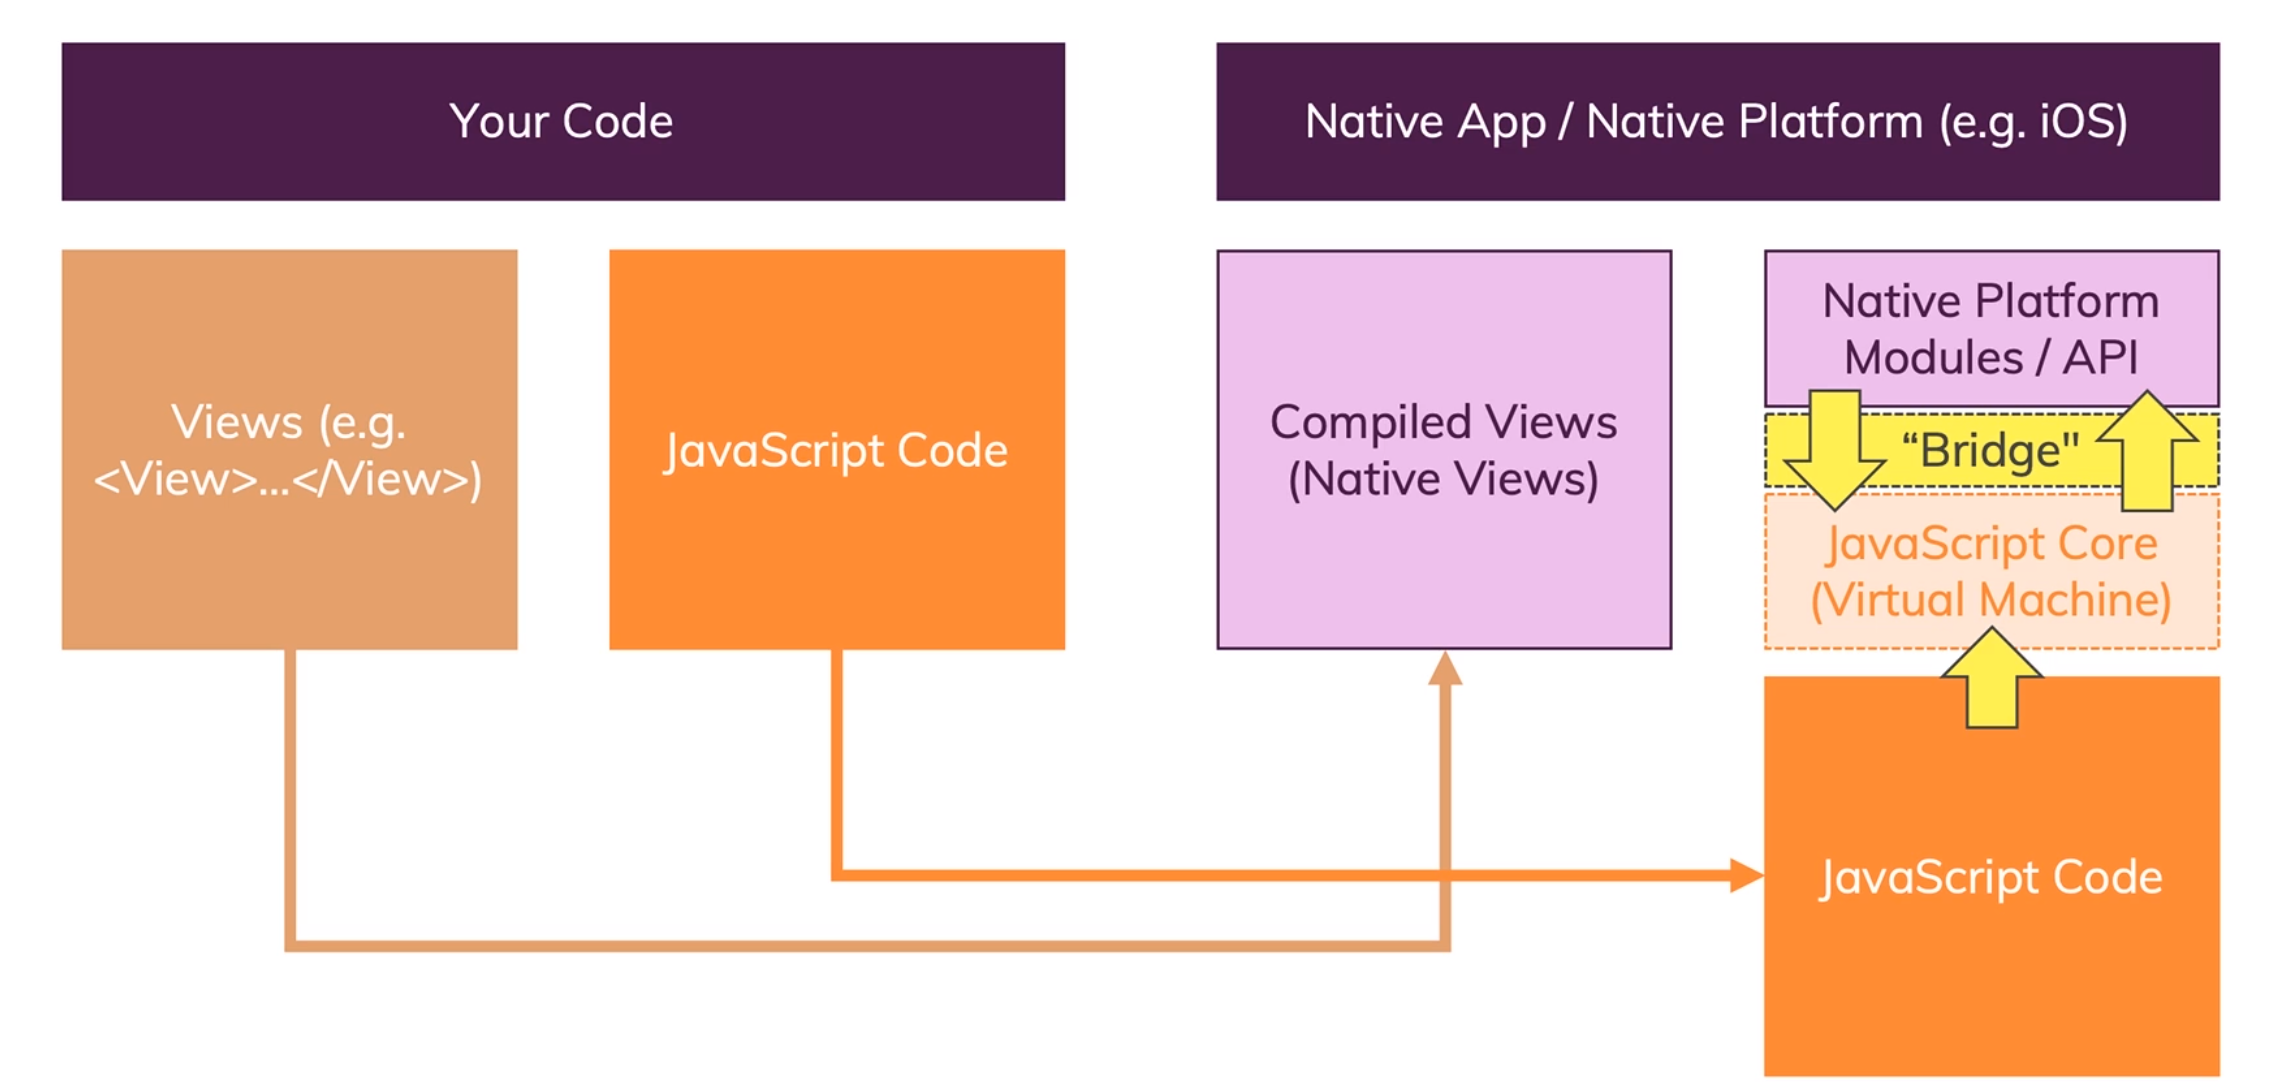
\includegraphics[width=15cm]{img/rn-working.png}
%  \caption{Ukážka fungovania React Native aplikácie}
%  \label{nativeappeg}
%\end{figure}	
\begin{figure}[!htbp]
  \centering  
  \def\stackalignment{c}
	\stackunder{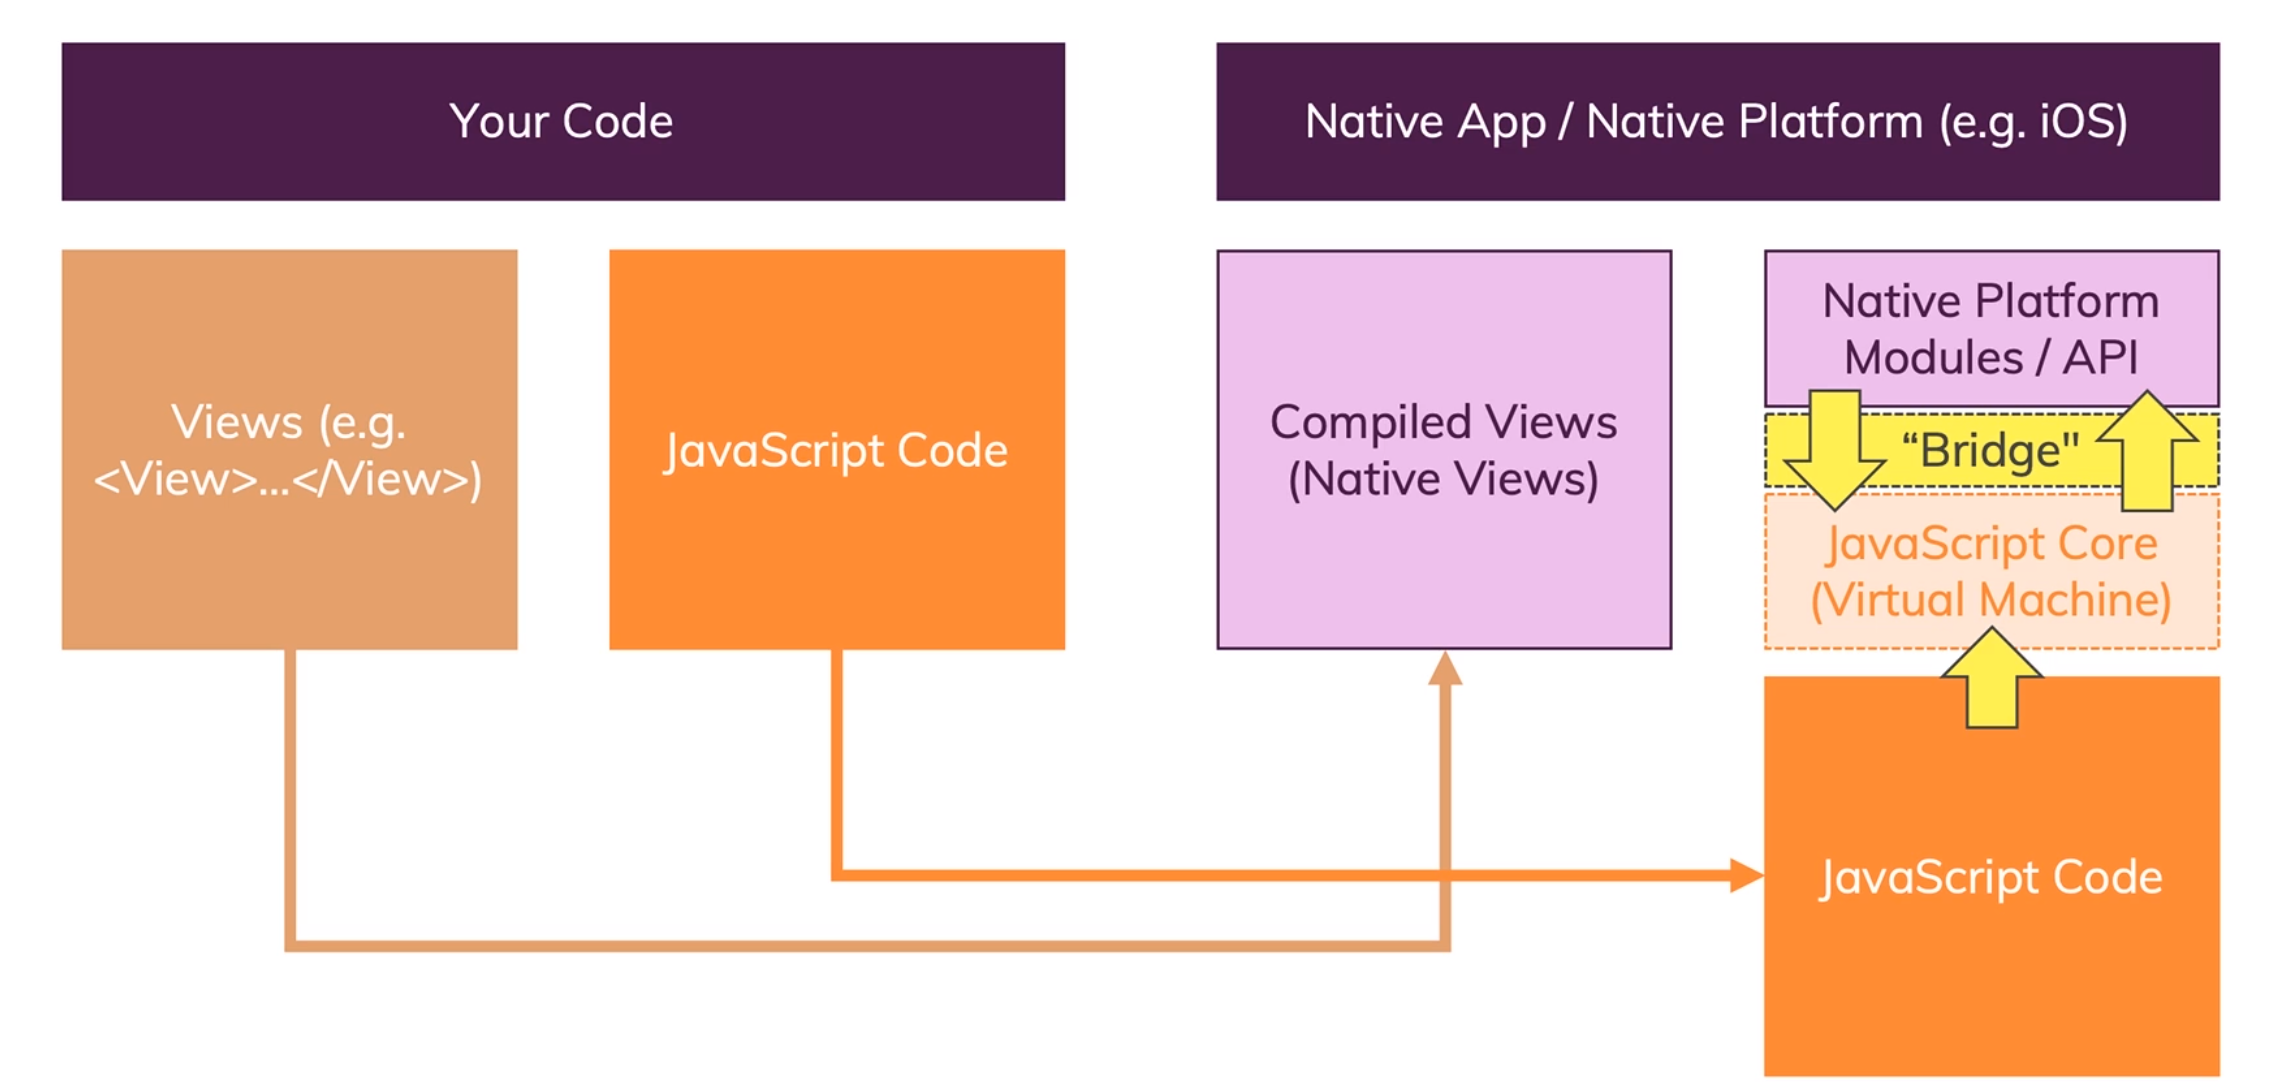
\includegraphics[width=15cm]{img/rn-working.png}}%
           {\scriptsize%
            Zdroj: \url{https://www.udemy.com/course/react-native-the-practical-guide/}}
	\caption{Ukážka fungovania React Native aplikácie}  
  \label{reactAppExplained}
\end{figure}
\subsubsection{Virtual DOM (Document Object Model)}
Ďalším dôležitým koncepotom v React Native, je tzv. Virtual DOM. Predtým, ako si vysvetlíme pracovanie s Virtual DOM v React Native, sa nato najprv pozrieme z pohľadu Reactu. DOM je vo všeobecnosti skratka pre Document Object Model (inak nazývaný aj real DOM), čo je programové rozhranie pre HTML a XML dokumenty. DOM reprezentuje dokument ako skupinu uzlov (tzv. "nodes") a objektov. To umožňuje jazykom ako napríklad JavaScript modifikovať dané uzly a tým aj celý dokument. DOM je reprezentovaný ako dátovy strom, vďaka čomu je každá zmena rýchla. Avšak po tejto zmene, zmenené elementy a ich potomkovia musia byť nanovo vyrendrované aby nastal aj priamo update UI danej aplikácie. Proces rendrovania je to, čo spôsobuje nezanedbateľné spomalenie výkonu, ktoré je navyše priamo úmerné so zväčšujúcim sa počtom UI komponentov, ktoré treba nanovo vyrendrovať.

Tu prichádza na scénu Virtual DOM a dosahuje podstatne lepšie výkonostné výsledky ako real DOM. Virtual DOM je iba virtuálne znázornenie DOM. Vždy, keď sa zmení stav aplikácie, namiesto real DOM sa aktualizuje virtual DOM. Keď je do UI pridaný nový element, vytvorí sa virtual DOM (reprezentovaný ako strom). Akonáhle sa zmení stav ktoréhokoľvek elementu, vytvorí sa nový virtual DOM, prebehne proces porovnania (nazývaný "diffing") aktuálnej verzie a prechádzajúcej verzie vritual DOM. Potom sa vypočíta najlepší možný spôsob ako tieto zmeny premietnuť do real DOM. Akonáhle React vie, ktoré elementy vo virtual DOM boli zmenené, zaktualizuje len dané elementy v real DOM. Vďaka tomu je výkon neporovnateľne lepší v porovnaní s priamou manipuláciou s DOM.

\begin{figure}[!htbp]
  \centering  
  \def\stackalignment{c}
	\stackunder{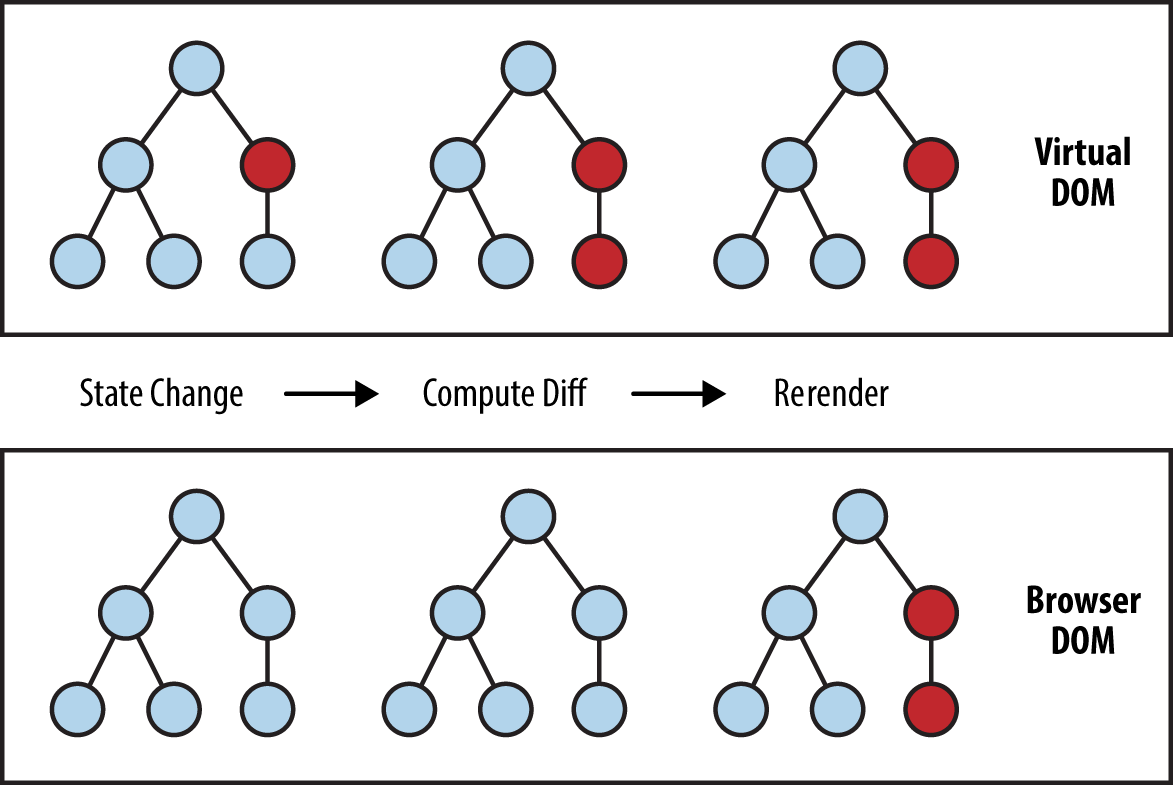
\includegraphics[width=12cm]{img/dom.png}}%
           {\scriptsize%
            Zdroj: \url{https://programmingwithmosh.com/react/react-virtual-dom-explained/}}
	\caption{Virtual DOM vs. real DOM}  
  \label{domImg}
\end{figure}
Na obrázku \ref{domImg} vidíme červené kruhy, ktoré znázorňujú zmenené uzly. Tieto uzly reprezentujú konkrétne UI elementy, ktorých stav sa zmenil. Následne je vypočítaný rozdiel medzi aktuálnou a predchádzajúcou verziou virtual DOM stromu, pričom celý podstrom rodiča je nanovo prerendrovaný a tým poskytne aktualizáciu UI. Aktualizácie real DOM sa posielajú hromadne, namiesto odosielania aktualizácií pre každú jednu zmenu stavu.

Spôsob akým virtual DOM využíva samotný React Native je vo veľkej miere podobný. Hlavnou odlišnosťou je, že sa namiesto webových komponentov rendrujú natívne komponenty, tým pádom sa nepoužívajú webové technológie.

\subsubsection{Základné komponenty}
Kľúčovým prvkom každej React Native aplikácie sú komponenty. Každý komponent má inú úlohu, no dokopy tvoria celok - samotnú aplikáciu. Z hľadiska koncepcie môžeme povedať, že komponenty sú podobné JavaScript funkciám. Vedia príjímať vstupy (nazývane ``props''), s ktorými potom umožňujú pracovať vo vnútri komponentu a vracajú elementy ktoré popisujú čo sa má zobraziť na obrazovke. V React Native existujú dva hlavné typy komponentov, ktoré tvoria aplikáciu. Sú štruktúrované rovnako, ako v bežnej webovej aplikácii vytvorenej pomocou Reactu.
\begin{itemize}[leftmargin=*]
{\bf \item Class komponenty} \newline
Sú to triedy rozširujúce základnú triedu z Reactu s názvom Component. Majú prístup k lifecycle metódam Reactu ako napríklad render či state/props funkcionalite od rodičovskej triedy. V súčasnosti sú menej používané kvôli tomu, že sú komplikovanejšie ako functional komponenty. Aj keď stále existujú prípady, v ktorých je ich syntax potrebná, vo všeobecnosti sa pri vytváraní nového komponentu viac používa syntax functional kompononetu. Vo výpise \ref{classComponent} máme úvedený aj jednoduchý príklad class komponentu.  \\

\begin{lstlisting}[  caption={Príklad class komponentu}, label={classComponent} ]
import React, { Component } from 'react';
import { Text } from 'react-native';

class Cat extends Component {
  render() {
    return (
      <Text>This is class component!</Text>
    );
  }
}

export default Cat;
\end{lstlisting}
{\bf \item Functional komponenty} \newline
Sú najjednoduchší spôsob vytvorenia komponentu. Ich deklarácia je v podstate rovnaká ako pri obyčajnej JavaScript funkcii. V minulosti sa za ich nevýhodu oproti class komponentom považovalo to, že neumožňovali správu stavov (states) a nemali prístup k lifecycle metódam ktoré React Native poskytuje. To sa zmenilo až po vydaní verzie 16.8.0 v roku 2019, v ktorej vývojári pridali Hooks, čím tento problém zanikol. Odvtedy sa ich popularita ešte zvýšila a stali sa novým štandartom. Na výpise \ref{funcComponent} môžeme vidieť, že je jednoduchšie ich udržiavať ``light weight'' a kód je pri nich čitateľnejší, ako pri class komponentoch. \\

\begin{lstlisting}[caption={Príklad function komponentu}, label={funcComponent}]
import React from 'react';
import { Text } from 'react-native';

const Cat = () => {
  return (
    <Text>This is functional component!</Text>
  );
}

export default Cat;
\end{lstlisting}

\end{itemize}

React Native navyše poskytuje aj sadu predpripravených hotových natívnych komponentov, ktoré sa dajú veľmi jednoducho použiť pri programovaní aplikácie. Patria medzi ne napríklad View, Text, Button, Image, či TextInput.

\subsubsection{Props a state}
Props a State sú dva typy dát, pomocou ktorých vieme pracovať s komponentami.
\begin{itemize}[leftmargin=*]
{\bf \item Props} \newline
Props (z anglického slova ``properties'') je obdoba argumentov pri klasických funkciách v JavaScripte alebo atribútov pri HTML. Komponenty prijímajú props od rodičovského komponentu. Ich dôležitou vlastnosťou je, že sú tzv. ``immutable'' tj. nemenné vo vnútri komponentu. V Reacte a v React Native smerujú dáta jedným smerom - od rodičovských komponentov k detským. Celý koncept props je založený natom, že si viete vytvoriť jeden komponent, ktorý je možné použiť na viacerých miestach v aplikácii. Rodičovské komponenty potom vedia zavolať váš vytvorený komponent, pričom na rôznych miestach vie mať rozličné props. Props v zásade pomáhajú písať znovu použiteľný kód.
{\bf \item State} \newline
State pracuje odlišne v porovnaní s props. Je to interná vlastnosť komponentu, ktorá pomáha v rámci komponentu sledovať určité informácie. Použitím ``setState'' sa daný komponent aj jeho detské komponenty nanovo vyrendrujú, vďaka čomu sa nemusí programátor zaoberať implementáciou event handlerov ako v iných jazykoch. State sa používa v situáciách, keď sa menia dáta v rámci komponentu. Dobrým príkladom je napríklad interakcia používateľa s komponentom, pri klikntí na tlačidlo alebo zaškrtnutí checkboxu. Napríklad pri vypĺňaní formuláru má každý z textových inputov svoj vlastný state. Ak vyplníte daný input, automaticky sa mení jeho state, čo spôsobuje prerendrovanie celého komponentu a všetkých jeho detskych komponentov. 
\end{itemize}
\subsubsection{Hooks}
Hooks boli predstavené vo verzii 16.8.0 v roku 2019. Ich hlavnou úlohou je umožniť používať state a lifecycle metódy vo functional komponentoch, čo predtým bolo možné iba vytvorením class komponentov (v nich Hooks nie sú použiteľné). Ich uvedenie výrazne zvýhodnilo používanie functional komponentov oproti class komponentom. Tak isto ako pri komponentoch, aj tu React Native umožňuje využiť predpripravené Hooks priamo od vývojárov. Najčastejšie používané sú useEffect a useState. V prípade potreby je možné si vytvoriť aj vlastný hook tak, aby spĺňal požadovanú funkcionalitu.
\subsection{Expo alebo React Native CLI ?}
Predtým ako sa programátor pustí do vývoja aplikácie pomocou React Native, ho čaká rozhodnutie či použiť pomocný framework Expo, alebo vstavanú funkcionalitu React Native CLI. Nato aby sme mohli vytvorenú aplikáciu vôbec spustiť, potrebujeme jednu z týchto technológii. \\



\subsubsection{Expo}
Framework používaný pri vytváraní React Native aplikácií. Je to balík nástrojov a služieb vytvorených pre React Native, ktoré pomáhajú pri vývoji aplikácie. \newline

{\bf Výhody}
\begin{itemize}
{\item Nevyžaduje vedomosť programovania v natívnom kóde.}
{\item Nepoužíva Xcode alebo Android Studio.} 
{\item Najrýchlejší a najjednoduchší spôsob, ako vytvoriť natívne React Native aplikácie.}
{\item Uvolňuje OTA updates.} 
{\item Vstavaný prístup k natívnym APIs.}
\end{itemize}

{\bf Nevýhody}
\begin{itemize}
{\item Ďalšia vrstva abstrakcie.} 
{\item Neumožňuje zasahovať do natívneho kódu.}
{\item Niesu k dispozicií všetky iOS a Android APIs.} 
\end{itemize}
\bigskip

\subsubsection{React Native CLI}
Vstavaný nástroj v React Native, ktorý pomáha spustiť aplikáciu. \newline

{\bf Výhody}
\begin{itemize}
{\item Umožňuje zasahovať do natívneho kódu.} 
{\item Vieme pomocou neho pridávať natívne moduly (Objective C/Java).} 
\end{itemize}

{\bf Nevýhody}
\begin{itemize}
{\item Vývoj iOS aplikácie nie je možný na inom OS ako MacOS.} 
{\item Na vytvorenie projektu sa vyžaduje Android Studio alebo XCode.}
{\item Nastavenie projektu (vrátane konfigurácie) je pomerne komplikované a nepohodlné.} 
{\item Neposkytuje niektoré JavaScript APIs napr. notifikácie, je potrebné ich ručne doinštalovať.}
\end{itemize}

\subsubsection{Odôvodnenie výberu}
V našom prípade sme si vybrali pracovať s Expom, keďže práca s ním je jednoduchšia a priamočiarejšia a vzhľadom na typ a vlastnosti aplikácie a jeho ostatné výhody, prevyšuje React Native CLI.

\section{Analytická časť}
\section{Návrhová časť}
\section{Implementačná časť}









